\documentclass[11pt,twocolumn]{scrartcl}
\usepackage[top=1cm, a4paper]{geometry}
\usepackage[utf8]{inputenc}
\usepackage[T1]{fontenc}
\usepackage[english]{babel}
\usepackage{csquotes}
\usepackage{biblatex}
\bibliography{literature}
\usepackage{amsmath}
\usepackage{amsfonts}
\usepackage{amssymb}
\usepackage{graphicx}
\author{Martin Unterreiner, 119981}
\title{Documentation Octopcous}
\begin{document}
\noindent
\maketitle
\section{Introduction}
Gestures for user interaction are predestined for mobile touchscreen devices like smartphones or tablet. On small devices it can be a frustrating experience for the users. It also can improve the collaboration for multi user application. Every user interactively follow the discussion.  Oliver Bau wanted to improve the gesture-based interface and provided an example of a dynamic guided gesture recognizer. In his work he combined an on-screen feedforward and feedback system to allow dynamically gestures in different direction. The user can evoke different commands, also the application remembers the way, it was performed. Therefore in OctoPocus a menu is shown with a press and wait gesture. When the user starts the gesture the progress is continuously updated until he finish. In the next section I will describe the feedforward and the Feedback mechanism.
\paragraph{Feedforward}
The feedforward mechanism gives the user an impression of the shape of the gesture. It also describes the command it is related. \citeauthor{Bau2008} uses predefined templates to represent the "gesture vocabulary". The starting points of all templates are the same and are initialized where the user tips the first time the screen with a "press and wait "gesture. 
 \begin{figure}
 	 \begin{center}
 	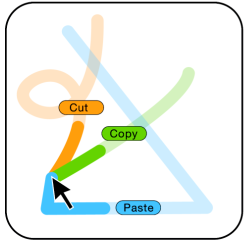
\includegraphics[scale=0.4]{./img/feedforward.png}
 	\caption{Feedforward.Bau and Mackay, 2008.}
 	 \end{center}
 \end{figure}
\paragraph{Feedback}
To provide the user a feedback, followed path is getting progressively thinner. With this gesture OctoPocus indicates that the application is recognizing is gesture. The progress of the gesture is calculated in realtime. \citeauthor{Bau2008} adapted in OctoPocus a version of \autocite{Rubine1991} algorithm. The gesture recognition is conducted by measuring the distance.
\begin{figure}[!h]
	\begin{center}
		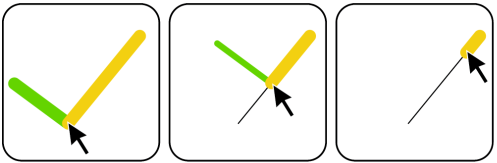
\includegraphics[scale=0.5]{./img/feedback.png}
		\caption{Feedback.Bau and Mackay, 2008.}
	\end{center}
\end{figure}
\section{My implementation}
In my first iteration I tried to implement a own implementation of Baus description within the dollar recognizer \footnote{https://github.com/olwal/dollar}. My first aim was to implement the menu and the recognizer with the main idea of feedforward and feedback. The second aim was to provide the execution of the command. Therefore I started to review the work of Juniior77 \footnote{https://github.com/Juniior77/Octopocus} and afterwards the MIS Project of Magdalena Keil and Jula McGibbon. 

In the beginning I started with the drawing and the implementation of the gesture recognizing. But after having problems with the implementation of the recognizer of Alex Olwal I have fallen back to implementation of Juniior77, Magdalena Keil and Jula McGibbon. Most of my actual work of this implementation is some refactoring. My core idea of my implementation was to provide the user a menu which should disappear during movement of the gesture. My application doesn't difference between a Novice or Expert mode nor it doesn't learn the gestures. In fact I wanted to provide the menu (feedforward) even after a release of the finger tip to prove the user some time to memories the different paths. 

\begin{figure}[!h]
	\label{fig:menu}
	\begin{center}
		\includegraphics[scale=0.3]{./img/myoctopocus.png}
		\caption{Menu with the feedforward path.}
	\end{center}
\end{figure}

\begin{figure}[!h]
		\label{fig:menu2}
	\begin{center}
		\includegraphics[scale=0.3]{./img/myoctopocus2.png}
		\caption{Menu with the decreased feedforward path.}
	\end{center}
\end{figure}

After starting the application is waiting for the first touch of the user. As soon as a onTouchEvent is recognized the menu with the feedforward paths is shown \ref{fig:menu}. The user can now follow one of the shown path. During the movement the menu is getting smaller. So during the action movement the actual position is saved. During the whole process the view within the painting is invalidated.  After releasing the screen the recognizer is called. If he recognize a path from the given template paths, it will print the result in a textview.
:w


%\nocite{*}
\printbibliography
\end{document}